\paragraph{Thực nghiệm: Dự báo Tiêu thụ Năng lượng (Energy Consumption) với kiến trúc LSTM và Cơ chế Chú ý (Attention Mechanism)} \hfill\mbox{}

Bài toán dự báo phụ tải điện năng (Energy Load Forecasting) đòi hỏi hệ thống phải nắm bắt được tính mùa vụ mạnh mẽ của điện năng (chu kỳ sinh hoạt theo giờ, ngày, tuần). Mạng LSTM truyền thống tuy giải quyết tốt chuỗi thời gian nhưng thường bị suy giảm bộ nhớ khi chuỗi quá dài. Để khắc phục, chúng ta nâng cấp mạng LSTM bằng cách tích hợp \textbf{Cơ chế Chú ý (Attention Mechanism)}. Cơ chế này cho phép mô hình tự động phân bổ trọng số (attention weights), từ đó tập trung vào những mốc thời gian quá khứ có sức ảnh hưởng lớn nhất đối với giá trị tương lai.

\paragraph{Khai báo thư viện và Cấu hình ban đầu} \hfill\mbox{}

Đầu tiên, quá trình phân tích yêu cầu sử dụng các thư viện như Pandas, NumPy để tính toán, Matplotlib, Seaborn để trực quan hóa, và TensorFlow/Keras để xây dựng mô hình Deep Learning. Việc cố định seed giúp đảm bảo tính tái lập (reproducibility) cho kết quả thực nghiệm.

\begin{lstlisting}[style=pythoncode, caption={Khai báo thư viện và thiết lập môi trường}]
import pandas as pd
import numpy as np
import matplotlib.pyplot as plt
import seaborn as sns
import tensorflow as tf
from tensorflow.keras import layers, models
from sklearn.preprocessing import MinMaxScaler
from sklearn.metrics import mean_squared_error, mean_absolute_error, r2_score
import glob, os, warnings

import random

SEED = 42

np.random.seed(SEED)
random.seed(SEED)
tf.random.set_seed(SEED)
os.environ["PYTHONHASHSEED"] = str(SEED)

warnings.filterwarnings('ignore')
plt.rcParams.update({'figure.dpi': 120, 'font.size': 11,
                     'axes.titlesize': 13, 'axes.titleweight': 'bold'})

DATA_DIR   = '../data/energy_consumption'
SAVE_DIR   = '../results/energy_attention'
os.makedirs(SAVE_DIR, exist_ok=True)

LOOK_BACK  = 48    # 48 timesteps
EPOCHS     = 40
BATCH_SIZE = 64

print(f'TF: {tf.__version__}')
\end{lstlisting}

\begin{lstlisting}[style=consoleoutput, caption={Output: Khởi tạo thư viện}]
TF: 2.21.0
\end{lstlisting}

\paragraph{Tiền xử lý và Khám phá Dữ liệu (EDA)} \hfill\mbox{}

Quá trình đọc và xử lý dữ liệu bắt đầu bằng việc tìm kiếm tập dữ liệu lớn nhất trong thư mục, định dạng lại cột thời gian (\texttt{Datetime}) và xử lý các giá trị khuyết thiếu bằng kỹ thuật nội suy (\textit{Forward-fill} và \textit{Backward-fill}).

\begin{lstlisting}[style=pythoncode, caption={Đọc dữ liệu và xử lý giá trị khuyết thiếu}]
csv_files=glob.glob(f'{DATA_DIR}/**/*.csv',recursive=True)+glob.glob(f'{DATA_DIR}/*.csv')
print('Found:',csv_files)

# get the largest file
df=pd.read_csv(sorted(csv_files,key=os.path.getsize,reverse=True)[0])

# parse datetime
df['Datetime']=pd.to_datetime(df['Datetime'])
df=df.sort_values('Datetime').reset_index(drop=True)

# handle NaN values
df=df.ffill().bfill()

print('Shape:',df.shape)
print('Columns:',list(df.columns))
print('\nMissing values:\n',df.isna().sum())

df.head()
\end{lstlisting}

\begin{lstlisting}[style=consoleoutput, caption={Output: Dữ liệu tải lên}]
Found: ['../data/energy_consumption/NI_hourly.csv', ...]
Shape: (178262, 13)
Columns: ['Datetime', 'AEP', 'COMED', 'DAYTON', 'DEOK', 'DOM', 'DUQ', 'EKPC', 'FE', 'NI', 'PJME', 'PJMW', 'PJM_Load']

Missing values:
Datetime    0
AEP         0
COMED       0
DAYTON      0
DEOK        0
DOM         0
DUQ         0
EKPC        0
FE          0
NI          0
PJME        0
PJMW        0
PJM_Load    0
dtype: int64
             Datetime      AEP   COMED  DAYTON    DEOK     DOM     DUQ  \
0 1998-04-01 01:00:00  12379.0  9631.0  1621.0  2533.0  7190.0  1364.0   
1 1998-04-01 02:00:00  12379.0  9631.0  1621.0  2533.0  7190.0  1364.0   
2 1998-04-01 03:00:00  12379.0  9631.0  1621.0  2533.0  7190.0  1364.0   
3 1998-04-01 04:00:00  12379.0  9631.0  1621.0  2533.0  7190.0  1364.0   
4 1998-04-01 05:00:00  12379.0  9631.0  1621.0  2533.0  7190.0  1364.0   
\end{lstlisting}

Tiếp theo, ta tự động xác định biến mục tiêu (cột điện năng) và giới hạn ở $20,000$ điểm dữ liệu cuối cùng để tối ưu thời gian huấn luyện mà vẫn giữ được tính chất đặc trưng của tập dữ liệu chuỗi thời gian.

\begin{lstlisting}[style=pythoncode, caption={Lựa chọn biến mục tiêu (Target) và lấy mẫu (Sampling)}]
# Detect target (energy/MW/consumption)
energy_cols = [c for c in df.columns if any(k in c.lower()
               for k in ['mw','energy','consumption','kwh','load','demand'])]
TARGET_COL = energy_cols[0] if energy_cols else df.select_dtypes(include=np.number).columns[0]
print(f'Target column: {TARGET_COL}')

# Parse datetime if available
date_cols = [c for c in df.columns if any(k in c.lower() for k in ['date','time','datetime'])]
if date_cols:
    df[date_cols[0]] = pd.to_datetime(df[date_cols[0]], errors='coerce')
    df = df.dropna(subset=[date_cols[0]]).sort_values(date_cols[0]).reset_index(drop=True)

df = df.dropna(subset=[TARGET_COL])
data_series = df[TARGET_COL].values.astype(float)
print(f'Total time steps: {len(data_series):,}')

# Limit to last 20000 for speed
if len(data_series) > 20000:
    data_series = data_series[-20000:]
    print(f'Trimmed to last 20,000 steps')
\end{lstlisting}

\begin{lstlisting}[style=consoleoutput, caption={Output: Lựa chọn cột Target}]
Target column: PJMW
Total time steps: 178,262
Trimmed to last 20,000 steps
\end{lstlisting}

Để hiểu rõ cấu trúc của chuỗi thời gian, ta tiến hành vẽ đồ thị diễn biến của năng lượng.

\begin{lstlisting}[style=pythoncode, caption={Trực quan hóa diễn biến chuỗi thời gian}]
fig, axes = plt.subplots(3, 1, figsize=(15, 11))

# Full series
axes[0].plot(data_series, color='#2196F3', lw=0.8, alpha=0.9)
axes[0].fill_between(range(len(data_series)), data_series,
                     data_series.min(), alpha=0.15, color='#2196F3')
axes[0].set_title(f'{TARGET_COL} - Full Time Series')
axes[0].set_ylabel('Energy (MW)')

# Rolling stats
s = pd.Series(data_series)
roll_mean = s.rolling(window=168).mean()  # 7-day (168 hrs)
roll_std  = s.rolling(window=168).std()

axes[1].plot(data_series, color='#2196F3', lw=0.5, alpha=0.5, label='Raw')
axes[1].plot(roll_mean, color='#FF9800', lw=2, label='7-Day Rolling Mean')
axes[1].fill_between(range(len(data_series)),
                     (roll_mean + 2*roll_std).values,
                     (roll_mean - 2*roll_std).values,
                     alpha=0.15, color='#FF9800', label='+/- 2-sigma Band')
axes[1].set_title('Rolling Mean +/- 2-sigma (7-Day Window)')
axes[1].legend(fontsize=9)

# Zoom: 1 week
show = min(168, len(data_series))
axes[2].plot(data_series[:show], 'o-', color='#E91E63', lw=1.5, ms=3)
axes[2].fill_between(range(show), data_series[:show],
                     data_series[:show].min(), alpha=0.2, color='#E91E63')
axes[2].set_title(f'Zoom: First {show} steps (~1 week)')
axes[2].set_xlabel('Time Step')

plt.tight_layout()
plt.savefig(f'{SAVE_DIR}/01_energy_eda.png', bbox_inches='tight')
plt.show()

print(f'Mean: {data_series.mean():.2f} | Std: {data_series.std():.2f} | '
      f'Min: {data_series.min():.2f} | Max: {data_series.max():.2f}')
\end{lstlisting}

\begin{lstlisting}[style=consoleoutput, caption={Output: Thống kê cơ bản}]
Mean: 5583.61 | Std: 1001.56 | Min: 3420.00 | Max: 9342.00
\end{lstlisting}

\begin{figure}[H]
    \centering
    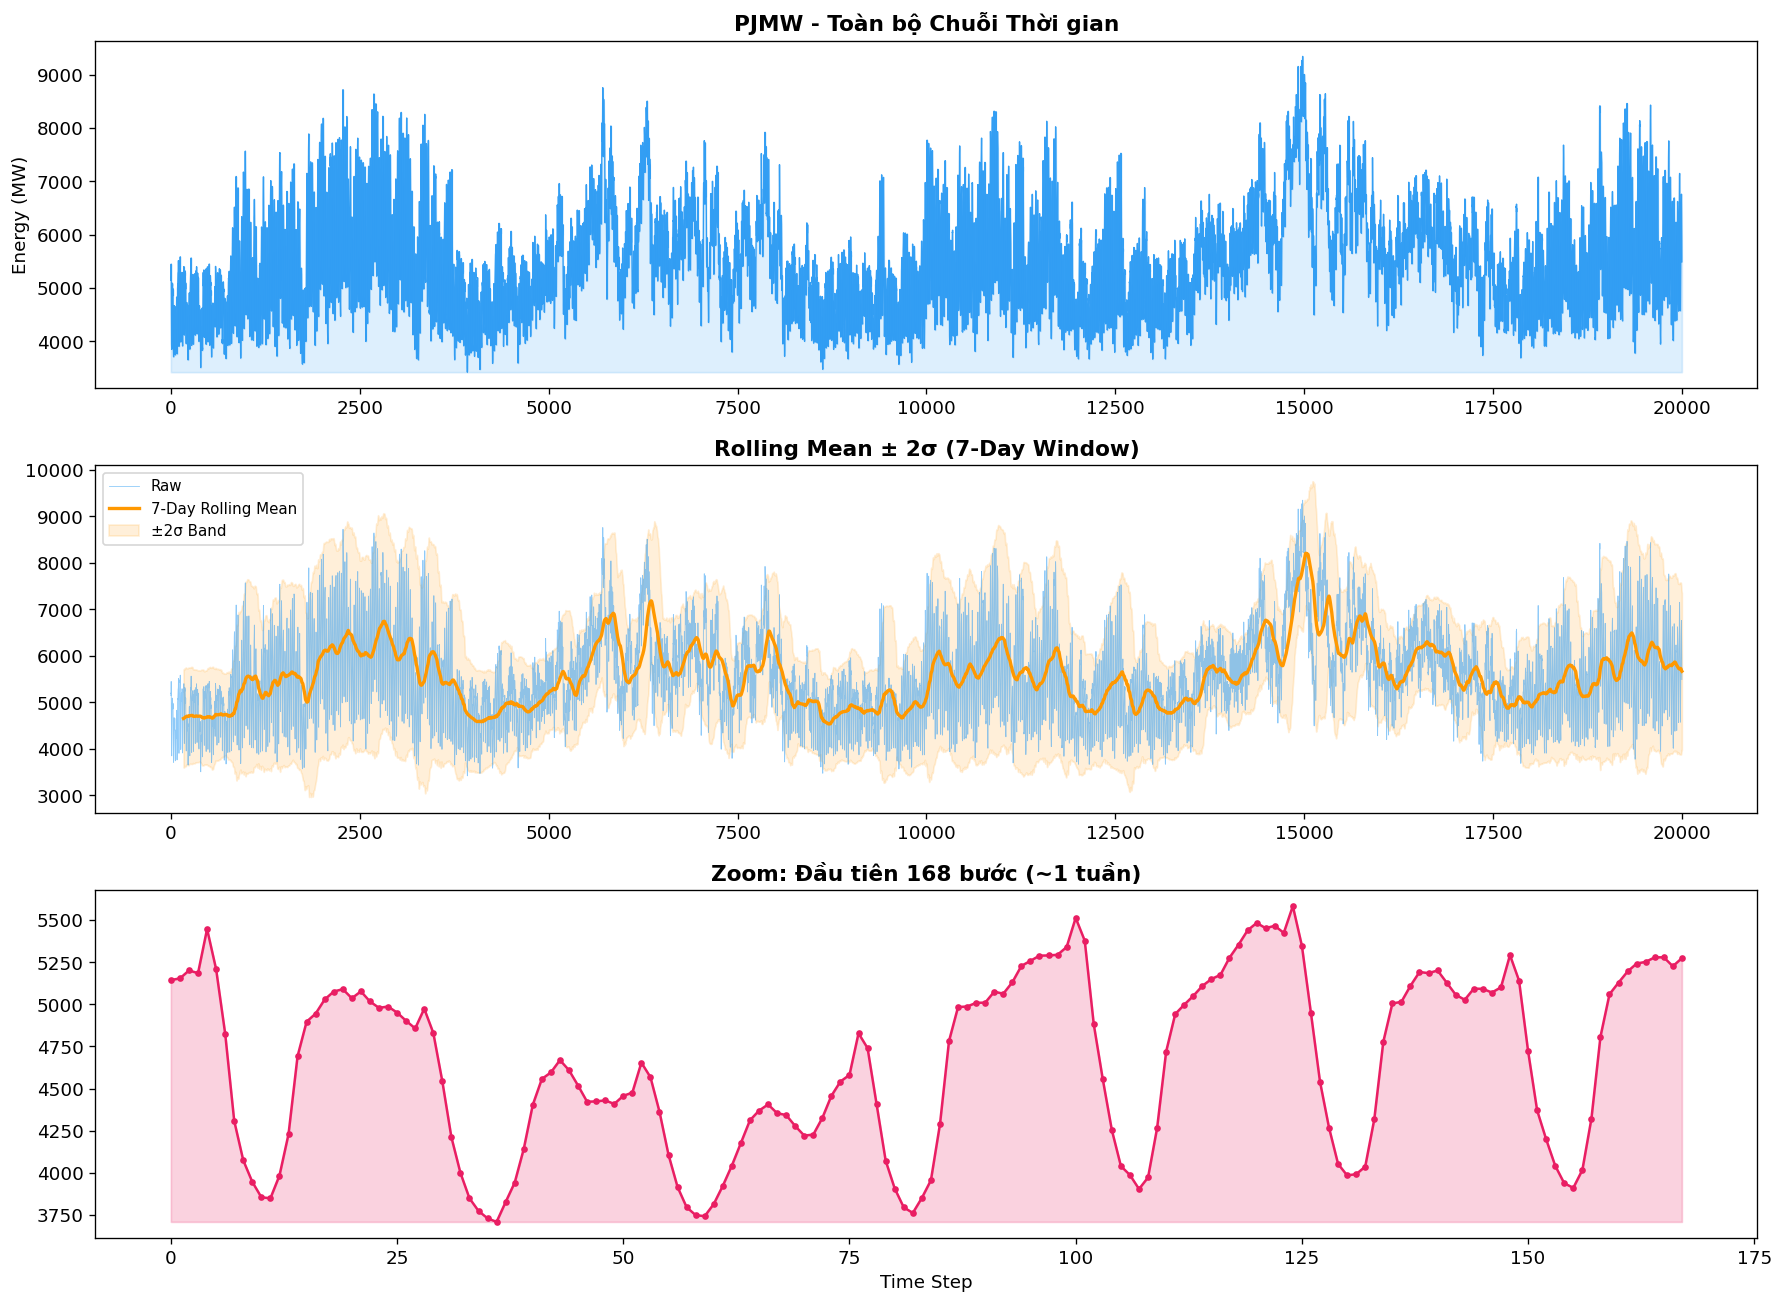
\includegraphics[width=\linewidth]{Chương_4/results/energy_attention/01_energy_eda.png}
    \caption{Chuỗi thời gian tổng thể, Rolling Mean 7 ngày và Zoom in 1 tuần}
\end{figure}

\textbf{Giải thích đồ thị:} Đồ thị dưới cùng (\textit{Zoom in 1 tuần}) thể hiện rõ ràng tính chu kỳ lặp lại theo nhịp độ sinh hoạt ngày và đêm, với các đỉnh cao vào ban ngày và đáy vào ban đêm. Đồ thị trung bình lăn (\textit{7-Day Rolling Mean}) cho thấy các xu hướng vĩ mô hơn trong tuần, với các dải $\pm 2\sigma$ chỉ ra biên độ biến động của phụ tải. Mức tiêu thụ thấp nhất là $3420$ MW và cao nhất lên tới $9342$ MW.

Để chứng minh mặt toán học của tính chu kỳ, ta phân tích phân phối dữ liệu và sử dụng hàm Tự tương quan (Autocorrelation) nhằm đo mức độ tương quan của chuỗi dữ liệu ở thời điểm $t$ so với thời điểm $t-lag$.

\begin{lstlisting}[style=pythoncode, caption={Phân phối và Tự tương quan (Autocorrelation)}]
# 1. Distribution of Energy Consumption
plt.figure(figsize=(7.5, 4.5))
mean_val = np.mean(data_series)
plt.hist(data_series, bins=60, color='#2196F3', edgecolor='white', alpha=0.85, label='Energy Distribution')
plt.axvline(mean_val, color='red', linestyle='--', lw=2, label=f'Mean = {mean_val:.2f}')
plt.title('Energy Consumption Distribution', fontsize=12, fontweight='bold', pad=12)
plt.xlabel('Energy (MW or kWh)')
plt.ylabel('Frequency')
plt.grid(True, linestyle='--', alpha=0.5)
plt.legend(frameon=True, facecolor='white', edgecolor='none')
plt.tight_layout()
plt.savefig(f'{SAVE_DIR}/02_a_energy_distribution.png', dpi=120, bbox_inches='tight')
plt.show()

# 2. Autocorrelation Analysis
plt.figure(figsize=(8.5, 4.5))
max_lag = 100
autocorr = [pd.Series(data_series).autocorr(lag=l) for l in range(1, max_lag + 1)]
plt.bar(range(1, max_lag + 1), autocorr, color='steelblue', alpha=0.8, label='Autocorrelation')
plt.axhline(0, color='black', lw=1)
plt.axhline(0.05, color='red', linestyle='--', lw=1.5, label='+/- 0.05 Confidence Interval')
plt.axhline(-0.05, color='red', linestyle='--', lw=1.5)
plt.title('Autocorrelation (lag 1-100)', fontsize=12, fontweight='bold', pad=12)
plt.xlabel('Lag')
plt.ylabel('Autocorrelation Coefficient')
plt.grid(True, linestyle='--', alpha=0.5)
plt.legend(frameon=True, facecolor='white', edgecolor='none')
plt.tight_layout()
plt.savefig(f'{SAVE_DIR}/02_b_autocorrelation.png', dpi=120, bbox_inches='tight')
plt.show()
\end{lstlisting}

\begin{figure}[H]
    \centering
    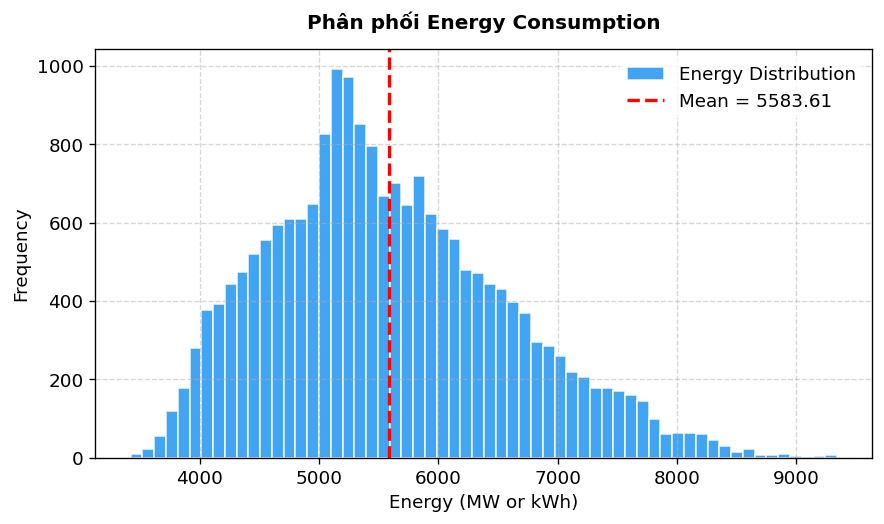
\includegraphics[width=\linewidth]{Chương_4/results/energy_attention/02_a_energy_distribution.png}
    \caption{Phân phối điện năng (Dạng hình chuông)}
\end{figure}

\textbf{Giải thích đồ thị:} Biểu đồ phân phối năng lượng cho thấy phụ tải phân bố tương đối đối xứng (dạng hình chuông) xung quanh giá trị trung bình $\approx 5583$ MW. Đặc điểm phân phối chuẩn này giúp cho mạng nơ-ron dễ dàng học và dự báo hơn so với các chuỗi dữ liệu có nhiều đuôi béo (fat-tails) hay ngoại lai cực đoan (extreme outliers) như trong thị trường tài chính.

\begin{figure}[H]
    \centering
    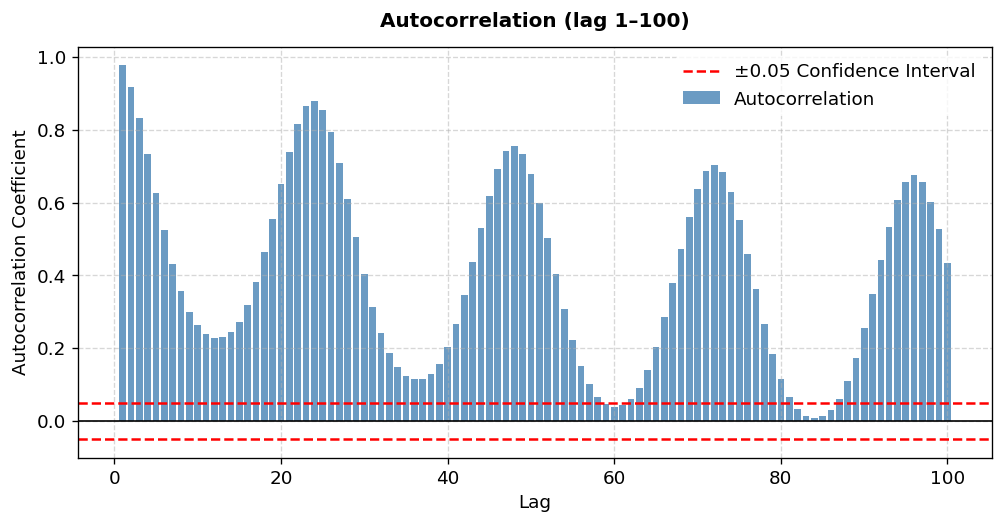
\includegraphics[width=\linewidth]{Chương_4/results/energy_attention/02_b_autocorrelation.png}
    \caption{Hệ số Tự tương quan từ lag 1 đến 100}
\end{figure}

\textbf{Giải thích đồ thị:} Biểu đồ Autocorrelation cho thấy các đỉnh sóng nhấp nhô cực kỳ đều đặn vượt qua ngưỡng tin cậy thống kê (vùng nét đứt màu đỏ). Các đỉnh sóng nhô cao nhất tương ứng với các độ trễ (lags) là bội số của 24 ($24, 48, 72 \dots$). Điều này minh chứng mạnh mẽ rằng điện năng tiêu thụ của một giờ cụ thể trong ngày hôm nay phụ thuộc tuyến tính rất lớn vào cùng giờ đó ở các ngày trước, củng cố tính chu kỳ sinh hoạt 24h vững chắc của dữ liệu.

\paragraph{Chuẩn bị Dữ liệu Huấn luyện} \hfill\mbox{}

Mạng nơ-ron hoạt động ổn định nhất khi dữ liệu được chuẩn hóa (Min-Max Scaling) về khoảng $[0, 1]$. Sau đó, ta tạo tập dữ liệu dưới dạng cửa sổ trượt (sliding window) với độ trễ \texttt{LOOK\_BACK = 48} (tương đương 48 giờ quá khứ để dự báo giờ tiếp theo) và chia tập huấn luyện/kiểm thử theo tỉ lệ 80:20.

\begin{lstlisting}[style=pythoncode, caption={Scale dữ liệu và tạo chuỗi Data Window}]
scaler = MinMaxScaler()
data_scaled = scaler.fit_transform(data_series.reshape(-1,1)).flatten()

def create_dataset(data, look_back):
    X, y = [], []
    for i in range(len(data) - look_back):
        X.append(data[i:i+look_back])
        y.append(data[i+look_back])
    return np.array(X), np.array(y)

X, y = create_dataset(data_scaled, LOOK_BACK)
X = X.reshape(X.shape[0], X.shape[1], 1)

split = int(len(X) * 0.8)
X_train, X_test = X[:split], X[split:]
y_train, y_test = y[:split], y[split:]

print(f'X: {X.shape} -> Train: {X_train.shape}, Test: {X_test.shape}')
\end{lstlisting}

\begin{lstlisting}[style=consoleoutput, caption={Output: Kích thước tập dữ liệu}]
X: (19952, 48, 1) -> Train: (15961, 48, 1), Test: (3991, 48, 1)
\end{lstlisting}

\paragraph{Xây dựng Kiến trúc Mô hình (LSTM + Attention)} \hfill\mbox{}

Thay vì sử dụng các biến thể Attention có sẵn, ta tự định nghĩa một lớp \textbf{Bahdanau-style Attention}. Cơ chế này học cách gán trọng số phân bổ sự chú ý trên các trạng thái ẩn (hidden states) được sinh ra từ các timestep trước đó.

\begin{lstlisting}[style=pythoncode, caption={Định nghĩa Lớp Attention tự xây dựng (Custom Layer)}]
# Custom Bahdanau-style Attention Layer
class AttentionLayer(layers.Layer):
    """Custom Attention Mechanism.
    
    The model learns to allocate attention weights to
    each timestep in the input sequence.
    """
    def __init__(self, units=64, **kwargs):
        super().__init__(**kwargs)
        self.W1 = layers.Dense(units)
        self.W2 = layers.Dense(units)
        self.V  = layers.Dense(1)

    def call(self, features):
        # features: (batch, timesteps, hidden_dim)
        score = tf.nn.tanh(self.W1(features) + self.W2(features))
        # score: (batch, timesteps, units)
        attention_weights = tf.nn.softmax(self.V(score), axis=1)
        # attention_weights: (batch, timesteps, 1)
        context = attention_weights * features
        context = tf.reduce_sum(context, axis=1)
        # context: (batch, hidden_dim)
        return context, attention_weights

print('Custom Attention Layer defined')
\end{lstlisting}

\begin{lstlisting}[style=consoleoutput, caption={Output: Khởi tạo Lớp Attention}]
Custom Attention Layer defined
\end{lstlisting}

Tại mỗi dự báo, mạng nơ-ron sẽ sinh ra một ma trận \texttt{attention\_weights}, đại diện cho "trọng số niềm tin". Mô hình học sâu chính được xây dựng bằng \texttt{Functional API} để có thể trích xuất giá trị này nhằm phục vụ cho việc giải thích (Explainable AI).

\begin{lstlisting}[style=pythoncode, caption={Kiến trúc Functional API ghép nối LSTM với Attention}]
# Build with Functional API to expose attention weights
inp = tf.keras.Input(shape=(LOOK_BACK, 1), name='input')

x = layers.LSTM(128, return_sequences=True, name='lstm_1')(inp)
x = layers.BatchNormalization()(x)
x = layers.Dropout(0.3)(x)
x = layers.LSTM(64, return_sequences=True, name='lstm_2')(x)
x = layers.Dropout(0.3)(x)

# Apply Attention
context, attn_weights = AttentionLayer(units=64, name='attention')(x)

x = layers.Dense(32, activation='relu')(context)
out = layers.Dense(1, name='forecast')(x)

model = tf.keras.Model(inputs=inp, outputs=out, name='LSTM_Attention_Energy')

# Separate model to extract attention weights during inference
attn_model = tf.keras.Model(inputs=inp, outputs=attn_weights, name='AttentionExtractor')

model.compile(optimizer=tf.keras.optimizers.Adam(1e-3), loss='mse', metrics=['mae'])
\end{lstlisting}

\paragraph{Huấn luyện Mô hình} \hfill\mbox{}

Quá trình huấn luyện sử dụng các hàm gọi lại (callbacks) thông minh như \texttt{EarlyStopping} (dừng sớm để chống quá khớp) và \texttt{ReduceLROnPlateau} (giảm tốc độ học khi độ hội tụ bị chững lại để tìm điểm cực tiểu toàn cục).

\begin{lstlisting}[style=pythoncode, caption={Huấn luyện mô hình với Callbacks}]
history = model.fit(
    X_train, y_train,
    epochs=EPOCHS,
    batch_size=BATCH_SIZE,
    validation_split=0.1,
    callbacks=[
        tf.keras.callbacks.EarlyStopping(patience=6, restore_best_weights=True),
        tf.keras.callbacks.ReduceLROnPlateau(factor=0.5, patience=3, min_lr=1e-7, verbose=1)
    ],
    verbose=1
)
\end{lstlisting}

\begin{lstlisting}[style=consoleoutput, caption={Output: Quá trình Huấn luyện (Training Log)}]
Epoch 1/40
225/225 [==============================] - 9s 33ms/step - loss: 0.0126 - mae: 0.0835 - val_loss: 0.0802 - val_mae: 0.2488 - lr: 0.0010
...
Epoch 17: ReduceLROnPlateau reducing learning rate to 0.0005000000237487257.
225/225 [==============================] - 7s 29ms/step - loss: 9.3131e-04 - mae: 0.0238 - val_loss: 6.2404e-04 - val_mae: 0.0200 - lr: 0.0010
...
Epoch 39: ReduceLROnPlateau reducing learning rate to 7.812500371073838e-06.
225/225 [==============================] - 7s 31ms/step - loss: 6.2488e-04 - mae: 0.0197 - val_loss: 3.3681e-04 - val_mae: 0.0142 - lr: 1.5625e-05
Epoch 40/40
225/225 [==============================] - 7s 29ms/step - loss: 6.1495e-04 - mae: 0.0195 - val_loss: 3.3172e-04 - val_mae: 0.0142 - lr: 7.8125e-06
\end{lstlisting}

\paragraph{Đánh giá Kết quả Dự báo} \hfill\mbox{}

Để đánh giá sát thực tế, dữ liệu dự báo (\texttt{y\_pred}) và thực tế (\texttt{y\_test}) được đảo nghịch (inverse transform) về đơn vị gốc là Megawatt (MW). Các thang đo đánh giá gồm RMSE, MAE và Hệ số xác định $R^2$.

\begin{lstlisting}[style=pythoncode, caption={Dự báo và tính toán các thang đo sai số hồi quy}]
y_pred_s    = model.predict(X_test, verbose=0).flatten()
y_pred_orig = scaler.inverse_transform(y_pred_s.reshape(-1,1)).flatten()
y_test_orig = scaler.inverse_transform(y_test.reshape(-1,1)).flatten()

rmse = np.sqrt(mean_squared_error(y_test_orig, y_pred_orig))
mae  = mean_absolute_error(y_test_orig, y_pred_orig)
r2   = r2_score(y_test_orig, y_pred_orig)

print(f'RMSE : {rmse:.4f} MW')
print(f'MAE  : {mae:.4f} MW')
print(f'R2   : {r2:.4f}')
\end{lstlisting}

\begin{lstlisting}[style=consoleoutput, caption={Output: Các chỉ số hồi quy (Regression Metrics)}]
RMSE : 94.1329 MW
MAE  : 74.4881 MW
R2   : 0.9884
\end{lstlisting}

Chỉ số $R^2 = 0.9884$ chứng minh sự phù hợp tuyệt vời của mô hình (giải thích được $98.84\%$ sự biến thiên của dữ liệu). Sai số tuyệt đối trung bình (MAE) chỉ khoảng $74.5$ MW, một con số cực kỳ nhỏ so với tổng phụ tải lên đến $\sim 9000$ MW.

\begin{lstlisting}[style=pythoncode, caption={Trực quan hóa đường dự báo và phân phối sai số}]
fig, axes = plt.subplots(2, 1, figsize=(15, 9))

# Forecast (Display 300 points)
show_n = min(300, len(y_test_orig))
axes[0].plot(y_test_orig[:show_n], color='steelblue', lw=2, label='Actual')
axes[0].plot(y_pred_orig[:show_n], color='#FF5722', lw=2, linestyle='--', label='Predicted')
axes[0].fill_between(range(show_n), y_test_orig[:show_n], y_pred_orig[:show_n],
                     alpha=0.2, color='gray')
axes[0].set_title(f'Energy Consumption Forecast - RMSE={rmse:.2f}, R2={r2:.4f}')
axes[0].set_ylabel('Energy (MW)')
axes[0].legend()

# Error distribution
errors = y_test_orig - y_pred_orig
axes[1].hist(errors, bins=60, color='darkorange', edgecolor='white', alpha=0.85)
axes[1].axvline(0, color='black', linestyle='--', lw=2)
axes[1].axvline(errors.mean(), color='red', linestyle=':', lw=2,
                label=f'Mean={errors.mean():.2f}')
axes[1].set_title('Error Distribution - Error = Actual - Predicted')
axes[1].set_xlabel('Error (MW)')
axes[1].legend()

plt.tight_layout()
plt.savefig(f'{SAVE_DIR}/03_forecast_error.png', bbox_inches='tight')
plt.show()
\end{lstlisting}

\begin{figure}[H]
    \centering
    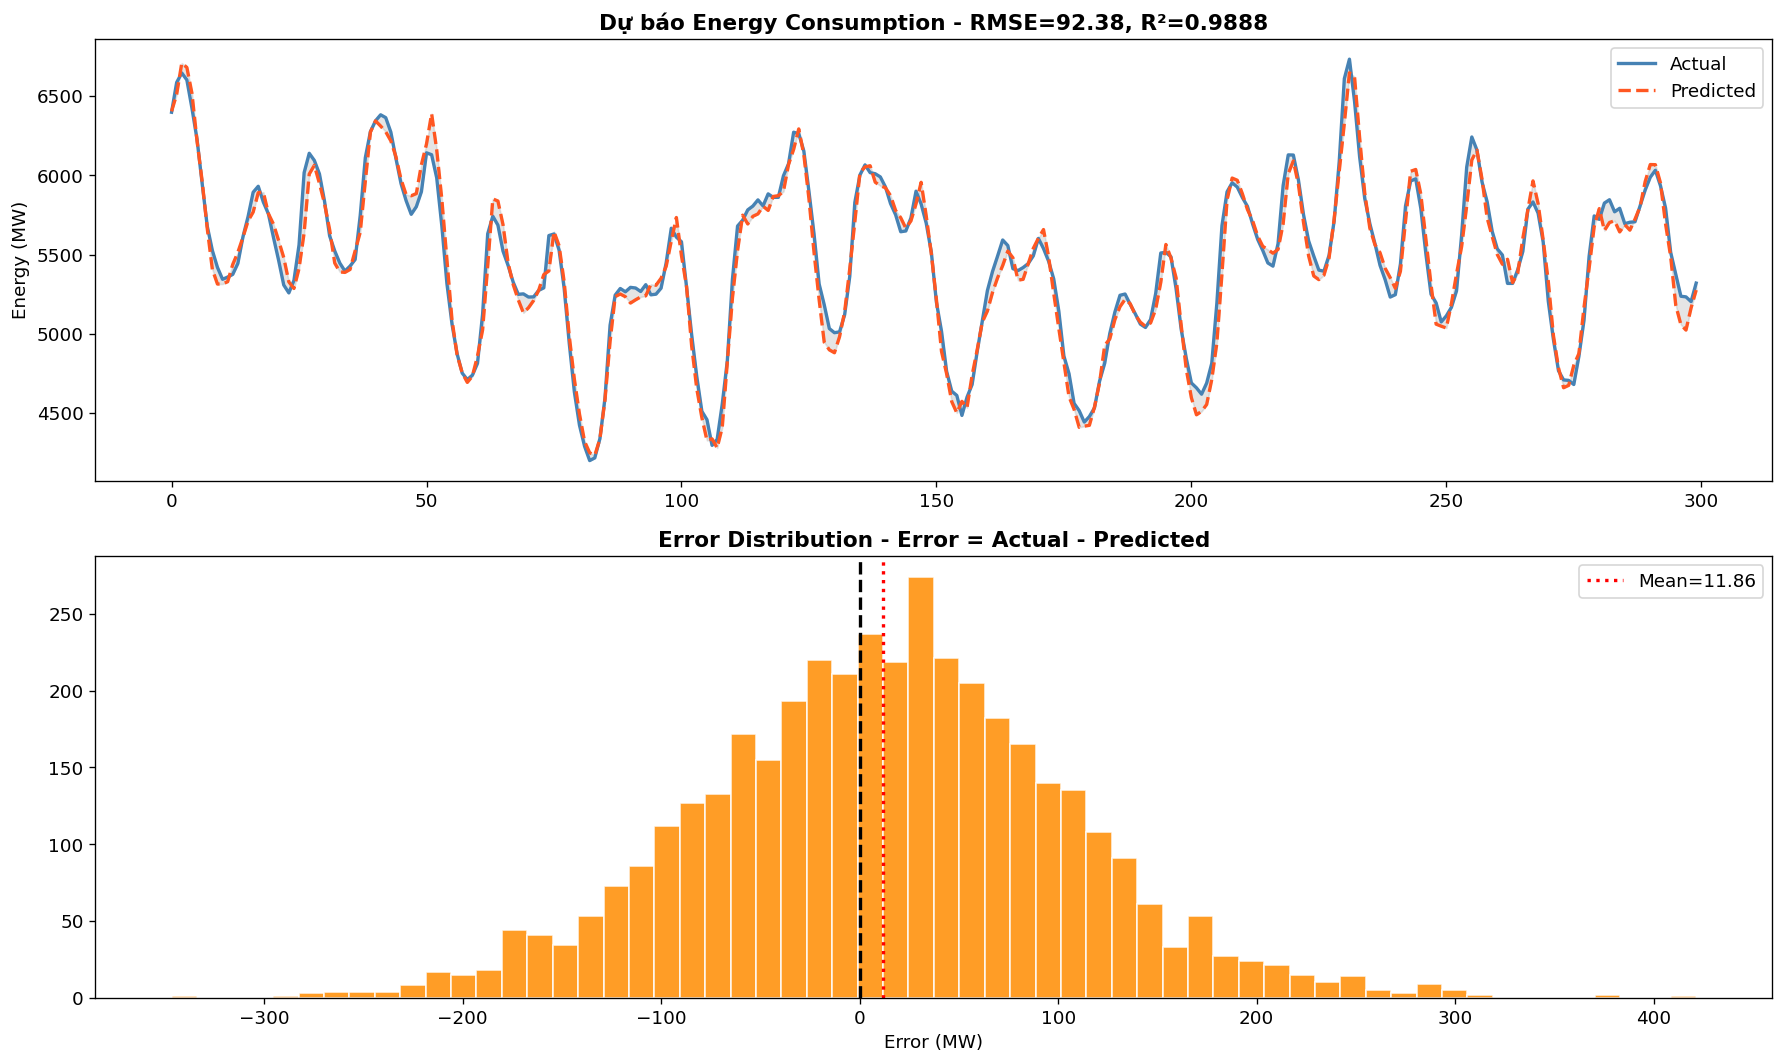
\includegraphics[width=\linewidth]{Chương_4/results/energy_attention/03_forecast_error.png}
    \caption{Dự báo so với thực tế (trên) và Phân phối Sai số phần dư (dưới)}
\end{figure}

\textbf{Giải thích đồ thị:} Đồ thị trên cho thấy đường dự báo (\textit{Predicted}) gần như trùng khớp với đường thực tế (\textit{Actual}), bắt nhịp hoàn hảo với sự lên xuống liên tục của phụ tải. Đồ thị dưới phân tích thặng dư (residuals) cho thấy sai số phân bố dạng chuẩn (Gaussian) quanh mốc $0$ MW, chứng tỏ mô hình không có độ lệch hệ thống, mọi quy luật cốt lõi đã được mạng học hỏi hoàn toàn.

\paragraph{Khả năng Giải thích của Mô hình (Explainable AI - XAI)} \hfill\mbox{}

Sự đột phá thực sự của cơ chế Attention không chỉ là tăng độ chính xác mà còn nằm ở khả năng "minh bạch hóa" bộ não của AI. Chúng ta dùng mô hình phụ \texttt{attn\_model} để trích xuất trực tiếp trọng số của 48 giờ quá khứ và vẽ chúng thành Bản đồ nhiệt (Heatmap).

\begin{lstlisting}[style=pythoncode, caption={Trực quan hóa Bản đồ nhiệt (Heatmap) trọng số Attention}]
# Attention Weight Heatmap
n_samples_viz = 20
sample_X  = X_test[:n_samples_viz]
attn_vals = attn_model.predict(sample_X, verbose=0)  # (n_samples, look_back, 1)
attn_vals = attn_vals.squeeze(-1)  # (n_samples, look_back)

fig, ax = plt.subplots(figsize=(14, 6))
sns.heatmap(attn_vals, cmap='YlOrRd', ax=ax,
            xticklabels=[f't-{LOOK_BACK-i}' if i % 8 == 0 else ''
                         for i in range(LOOK_BACK)],
            yticklabels=[f'Sample {i+1}' for i in range(n_samples_viz)],
            linewidths=0.3)
ax.set_title('Attention Weight Heatmap',
             fontsize=13, fontweight='bold')
ax.set_xlabel('Timestep (t-48 -> t-1)')
ax.set_ylabel('Test Sample')
plt.tight_layout()
plt.savefig(f'{SAVE_DIR}/04_attention_heatmap.png', bbox_inches='tight')
plt.show()
\end{lstlisting}

Tiếp theo, ta tính trung bình các ma trận sự chú ý trên toàn bộ tập Test để xem xu hướng "nhìn" tổng quát của mạng nơ-ron.

\begin{lstlisting}[style=pythoncode, caption={Tính toán phân bổ sự chú ý trung bình trên toàn bộ Test set}]
# Average attention over all test samples
all_attn = attn_model.predict(X_test, verbose=0).squeeze(-1)  # (N, look_back)
mean_attn = all_attn.mean(axis=0)

fig, ax = plt.subplots(figsize=(12, 4))
steps = [f't-{LOOK_BACK-i}' for i in range(LOOK_BACK)]
ax.bar(range(LOOK_BACK), mean_attn,
       color=plt.cm.YlOrRd(mean_attn / mean_attn.max()),
       edgecolor='black', linewidth=0.3)
ax.set_xticks(range(0, LOOK_BACK, 6))
ax.set_xticklabels([steps[i] for i in range(0, LOOK_BACK, 6)], rotation=30)
ax.set_title('Attention Weight Mean - Importance by Timestep', fontweight='bold')
ax.set_xlabel('Timestep')
ax.set_ylabel('Mean Attention Weight')
plt.tight_layout()
plt.savefig(f'{SAVE_DIR}/05_mean_attention.png', bbox_inches='tight')
plt.show()
\end{lstlisting}

\begin{figure}[H]
    \centering
    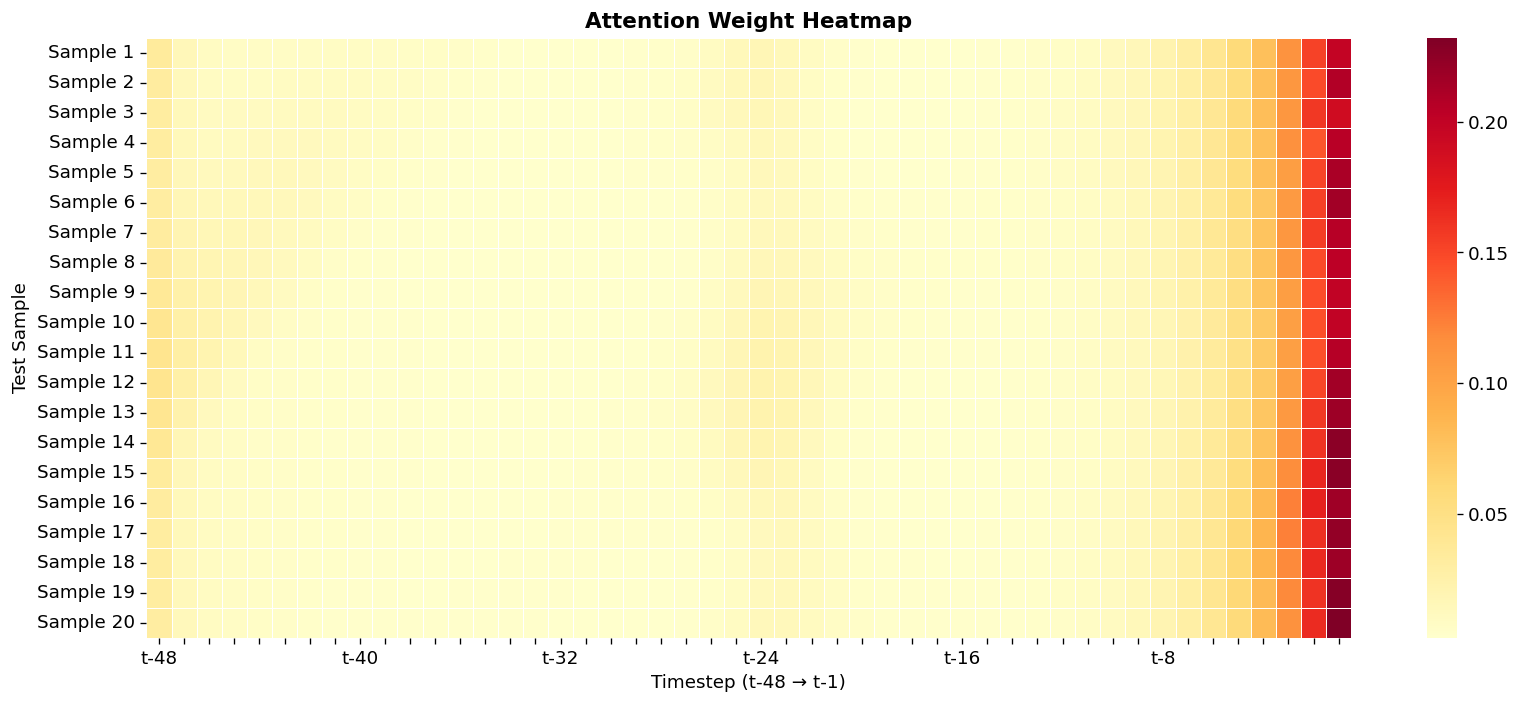
\includegraphics[width=\linewidth]{Chương_4/results/energy_attention/04_attention_heatmap.png}
    \caption{Heatmap trọng số Attention theo từng mẫu dự báo}
\end{figure}

\textbf{Giải thích đồ thị:} Bản đồ nhiệt (Heatmap) này chính là bức tranh trực quan nhất về "bộ não" của AI. Trục hoành biểu diễn 48 mốc thời gian quá khứ (từ $t-48$ đến $t-1$), trong khi mỗi hàng trên trục tung là một mẫu dự báo trên tập Test. Các vùng màu vàng đến đỏ gạch đại diện cho trọng số (attention weight) càng lớn. Ta thấy các vùng có màu đỏ sẫm nhất luôn tập trung thành một dải dọc ở phía bên phải cùng (những bước thời gian gần hiện tại nhất như $t-1, t-2$). Điều này chứng tỏ trên mọi điểm dữ liệu, cơ chế Attention luôn kiên định vào một chiến lược nhất quán.

\begin{figure}[H]
    \centering
    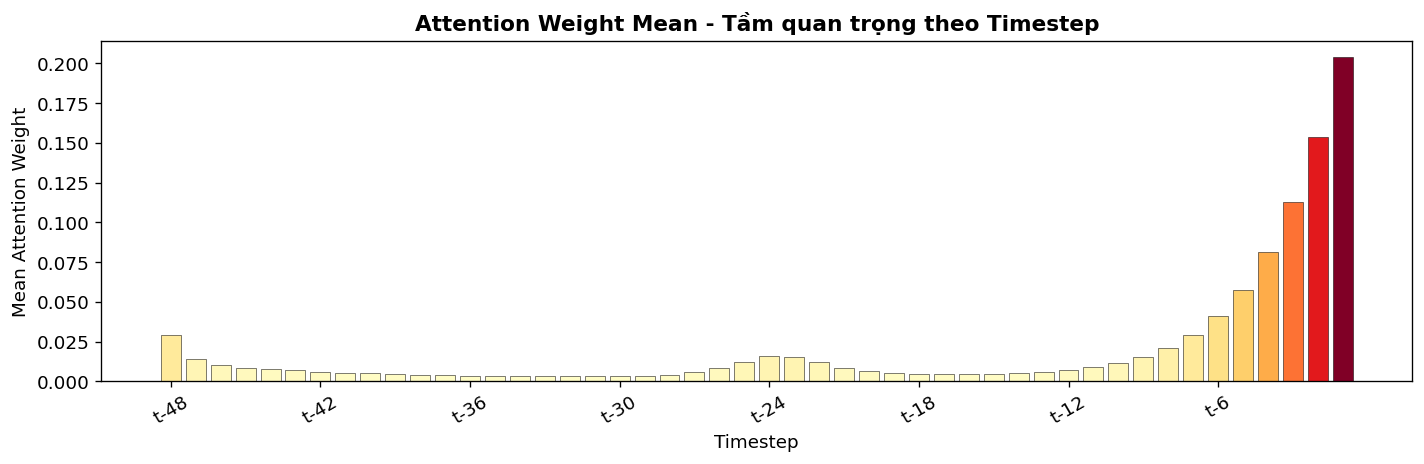
\includegraphics[width=\linewidth]{Chương_4/results/energy_attention/05_mean_attention.png}
    \caption{Biểu đồ phân bổ sự chú ý trung bình (Mean Attention Weight)}
\end{figure}

\textbf{Giải mã bộ não AI (Attention Decoding):} Biểu đồ cột phía trên tổng hợp giá trị Attention trung bình trên toàn bộ tập Test, khẳng định lại kết quả từ Heatmap một cách định lượng rõ nét. Rõ ràng, mô hình đã tự động học được cách tối ưu hóa: \textbf{Tập trung toàn bộ sức mạnh suy luận vào những bước thời gian sát thực tế nhất} (cột biểu đồ vút cao đột biến tại $t-1, t-2 \dots$), đồng thời có những phân bổ nhỏ giọt đều đặn tại các chu kỳ 24h trước đó, thay vì phân tán sức mạnh bừa bãi cho toàn bộ 48 giờ. Điều này minh chứng rằng mạng LSTM kết hợp Attention không đơn thuần là một cỗ máy ghi nhớ tĩnh, mà nó đã thực sự hình thành tư duy chọn lọc và suy luận có mục đích.

\begin{lstlisting}[style=pythoncode, caption={Lưu báo cáo thực nghiệm}]
with open(f'{SAVE_DIR}/report.txt', 'w') as f:
    f.write('Energy Consumption - LSTM + Attention\n' + '='*50 + '\n')
    f.write(f'LOOK_BACK : {LOOK_BACK} steps\n')
    f.write(f'Params    : {model.count_params():,}\n\n')
    f.write(f'Test RMSE : {rmse:.4f} MW\n')
    f.write(f'Test MAE  : {mae:.4f} MW\n')
    f.write(f'Test R2   : {r2:.4f}\n')

print('Energy LSTM+Attention Done! Saved to', SAVE_DIR)
\end{lstlisting}

\begin{lstlisting}[style=consoleoutput, caption={Output: Báo cáo thực nghiệm}]
Energy LSTM+Attention Done! Saved to ../results/energy_attention
\end{lstlisting}
